% !TEX program = xelatex

\documentclass[12pt,aspectratio=169,UTF8]{beamer}
\usefonttheme[onlymath]{serif}		
\usepackage{cqubeamer}  % cqu beamer template

\usepackage{ctex}
\setCJKfamilyfont{hwxk}{heiti}  

%\usepackage{xeCJK} %设置中文字体
%\setCJKmainfont{heiti} %xeCJK宏包下设置全局默认中文字体,默认为楷体STKaiti

\usepackage{amsmath,amsfonts,amssymb,bm}   % 数学公式字体宏包

\usepackage{xcolor}			               % 颜色宏包
\definecolor{cqu_blue}{RGB}{36,72,164}     % 自定义颜色
\usepackage{adjustbox}

\usepackage{listings}                      % 列表环境
\usepackage{verbatim}

\usepackage{subcaption}

\usepackage[listings]{tcolorbox}
\newtcbox{\mybox}{colback=red!5!white,colframe=green}
\tcbuselibrary{breakable}                  % tcolorbox 跨页显示
\usepackage{graphicx,url}

\usepackage{fontawesome}                   % 矢量图标库宏包
\usepackage{multicol}                      % 多栏显示宏包

\graphicspath{{figure/}} % 定义所有的图片文件在 figure目录下



\pdfbookmark[1]{CQU Beamer Template}{title} % "1" = section level,书签标题
\beamertemplatenavigationsymbolsempty

\title{强基转段面试汇报}
\author[陈骁睿]{\texorpdfstring{陈骁睿\\申请直博导师:张学锋}{陈骁睿}}
\date{\today}
\institute{重庆大学物理学院}
\begin{document}

% 标题页
\begin{frame}[plain]
  \begin{center}
      
\includegraphics[width=0.4\textwidth]{校徽+中英文校名_蓝色.pdf}
  \end{center}
  \titlepage
\end{frame}
\setcounter{framenumber}{0}

% % 目录页
\section*{}
\begin{frame}{目录}
  \begin{multicols}{2}
    \tableofcontents[subsubsectionstyle=hide]
  \end{multicols}
\end{frame}

% % 正文
\section{个人简介}
\subsection{基本信息}

\begin{frame}
  \frametitle{学习成绩}
    \begin{columns}
\begin{column}{0.4\textwidth}
\begin{table}[ht]
    \centering

    \label{tab:overall_performance}
    \begin{tabular}{cc}
        \hline
        \textbf{评价指标} & \textbf{成绩} \\
        \hline
        总绩点 & 3.4888 \\
        \hline
        年级参考排名 & 17 \\
        \hline
        专业参考排名 & 5 \\
        \hline
        班级参考排名 & 3 \\
        \hline
    \end{tabular}
        \caption{学习成绩总体情况}
\end{table}
\end{column}
\begin{column}{0.6\textwidth}
  \begin{figure}[!htbp]
\centering
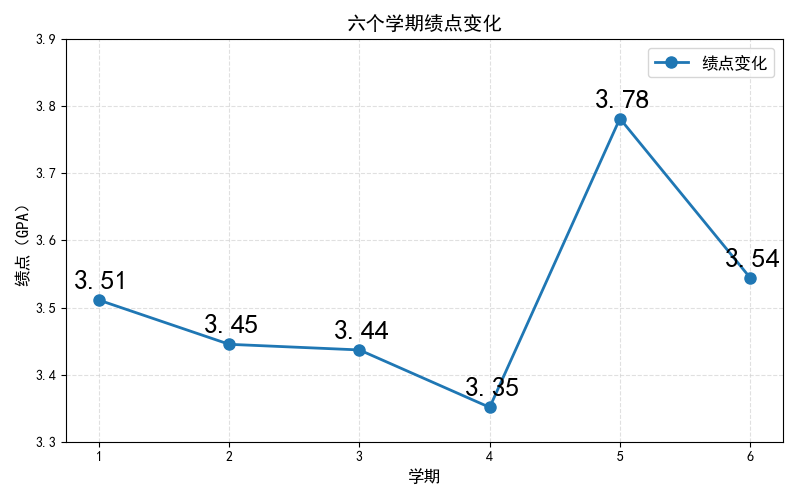
\includegraphics[width =\columnwidth]{GPAs.png}
% semesters = ['1', '2', '3', '4', '5', '6']  # 学期标签(简化为数字)
% gpa = [3.5111, 3.4452, 3.4368, 3.3512, 3.7818, 3.5444]  # 绩点数据
\caption{各学期绩点变化}
\label{fig:GPAs}
\end{figure}
\end{column}
\end{columns}
\end{frame}

\begin{frame}
  \frametitle{辅修计算机}
 \begin{figure}[ht]
    \centering
    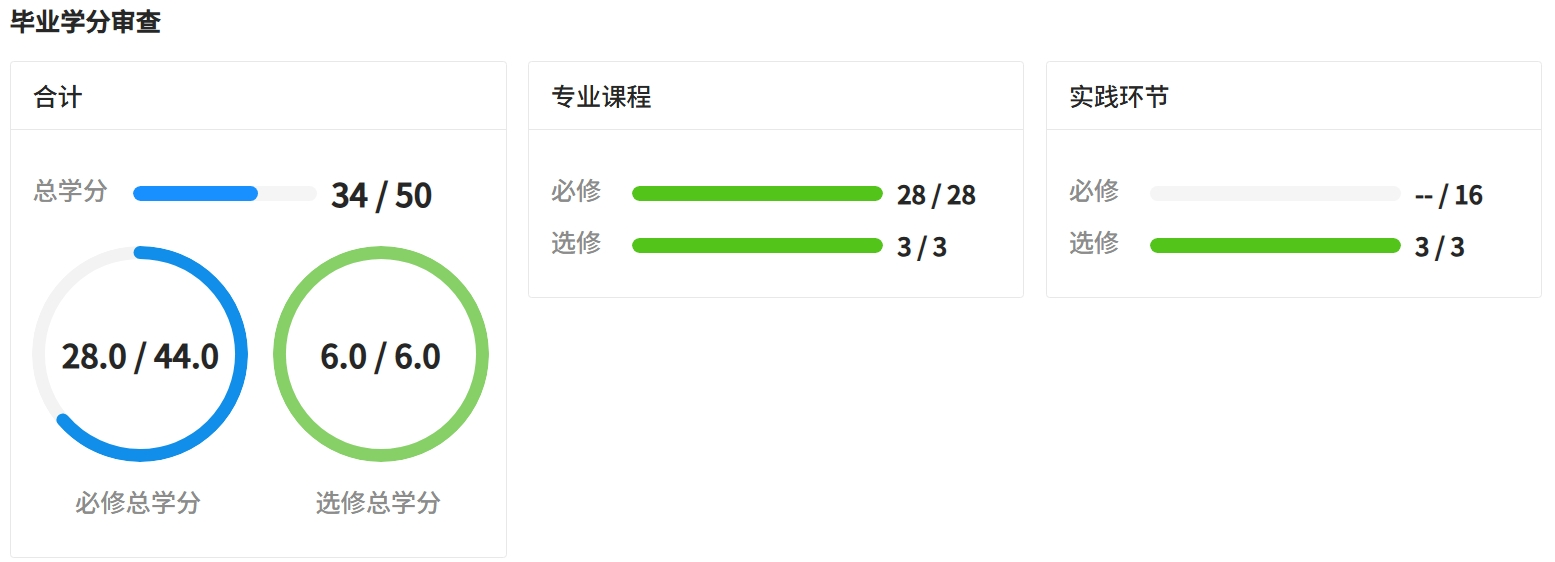
\includegraphics[width =.6\textwidth]{cs.jpeg}
    % \caption{计算机课程学分审查}
    \label{fig:cs}
\end{figure}
辅修计算机科学与技术。绩点:3.0764,学分已修够,只剩毕业设计,目标是拿到双学位。
  % \begin{itemize}
  %   \item 第一行
  %   \item 第二行
  % \end{itemize}
\end{frame}

\subsection{所获奖项}
\begin{frame}
  \frametitle{奖项}

  \begin{itemize}
   \item  重庆大学优异生
   \item   2022-2023第一学期,乙等奖学金
   \item   2022-2023第二学期,乙等奖学金
   \item   2022-2023第一学期,丙等奖学金
   \item   2024-2025第一学期,丙等奖学金
   \item   2022-2023学年,重庆大学优秀学生
   \item   2023-2024学年,优秀共青团员
   \item   蓝桥杯程序设计竞赛,重庆市一等奖
   \item   2025年美国大学生数学建模竞赛,成功参赛
   \item   第六届重庆市大学生物理创新竞赛,重庆市三等奖
   \item   第九届物理实验竞赛(创新)校赛,三等奖
   \item   第九届程序设计天梯赛校赛,三等奖
  \end{itemize}
\end{frame}

\section{科研经历}
\subsection{程序设计方面实践}
\begin{frame}
  \frametitle{较大型程序设计项目}
  \begin{itemize}
    \item 参与或独立完成多个较大型项目,包括:
    \begin{itemize}
      \item robmaster机甲大师机器人图像识别系统
      \item 高性能计算的并行算法设计
      \item 传统物联网java应用开发(计算机专业的课程设计)
    \end{itemize}
    \item 技术栈
    \begin{itemize}
      \item c++:cmake,VS,eigen,cuda
      \item data analysis:python,matlab,mathmatica
      \item machine learning:pytorch,openvino
      \item linux:bash,ubuntu,vim
      \item \LaTeX
    \end{itemize}
  \end{itemize}
\end{frame}

\subsection{量子蒙特卡洛算法的并行优化}
\begin{frame}
  \frametitle{量子蒙特卡洛算法的并行优化}
  \begin{itemize}
    \item 背景:量子蒙特卡洛随机级数展开算法难以并行化,存在性能瓶颈
    \item 目标:提高算法的并行计算效率
    \item 方法:通过CPU和GPU多核心(多线程)加速计算,优化算法结构
    \item 进展:已完成初步的程序实现,并进行了初步性能测试
    \item 结果:加速效果并不显著,在部分硬件上甚至出现了性能下降
    \item 改进:需要进一步性能分析,优化算法结构
  \end{itemize}
\end{frame}

\section{未来规划}
\subsection{未来规划}
\begin{frame}
  \frametitle{大四阶段}
  \begin{itemize}
    \item 课程方面:完成剩余课程,保持高绩点。在下学期提前学习研究生课程。
    \item 科研方面:继续量子蒙特卡洛算法的研究,并以此作为毕设题目。
    \item 计算机方面:完成计算机毕业设计,拿到双学位。
  \end{itemize}
\end{frame}

\begin{frame}
  \frametitle{博一到博二}
  \begin{itemize}
    \item 深入学习研究生课程,保持优异成绩。
    \item 继续完成量子蒙特卡洛算法的研究,发表第一篇论文。
  \end{itemize}
\end{frame}

\begin{frame}
  \frametitle{博三到博四}
  \begin{itemize}
    \item 在完成课程学习的基础上,全力投入科研工作。
    \item 强化物理理论基础,不局限于程序设计,提升科研能力。
    \item 在高水平期刊发表至少一篇论文。
    \item 在达到毕业要求的基础上,开始撰写毕业论文,争取提前毕业。
  \end{itemize}
\end{frame}

\appendix

\section*{backup}

\begin{frame}{结束}
  \vskip20pt
  \begin{center}
    \Huge{谢谢!\\ 欢迎批评指正!}
  \end{center}
  \vskip20pt
  \begin{table}
    \begin{tabular}{l}
      Chen Xiaorui (陈骁睿)                                                                                        \\
      {\color{blue}\faGraduationCap}\hspace{0.1cm}  Student of Physics, Chongqing University                    \\
      %\hspace{0.28cm} No.83 Shabei Street, Shapingba District \\
      {\color{blue}\faMapMarker}\hspace{0.28cm} Chongqing, 400045, P. R. China                                  \\
      {\color{blue}\faEnvelopeO}\hspace{0.1cm} {\href{mailto:20225847@stu.cqu.edu.cn}{20225847@stu.cqu.edu.cn}} \\
      {\color{blue}\faGithub}\hspace{0.1cm} {\href{https://github.com/XeriChen}{XeriChen}}                      \\
    \end{tabular}
  \end{table}%
  % \begin{picture}(0,0)
  %   \put(30,8){
\includegraphics[width=0.16\textwidth]{Wechat.png}}%
  % \end{picture}
\end{frame}

\end{document}
